\documentclass[xcolor=dvipsnames,aspectratio=169]{beamer}

% INCLUSIÓN DOS PAQUETES IMPRESCINDIBLES DE IDIOMA E CODIFICACIÓN DE CARACTERE.
\usepackage[T1]{fontenc}
\usepackage[english]{babel}
\usepackage[utf8]{inputenc}
\usepackage{csquotes}

%ACRONYMS para engadir un glosario de acronimos automatizado
% \usepackage[acronyms,nonumberlist,nopostdot,nomain,nogroupskip]{glossaries}
% \input{./acronyms.tex}

% PAQUETES PARA FIGURAS E GRAFICOS
\usepackage{graphicx}
%   \usepackage[pdftex]{graphicx}
  \usepackage{epstopdf}
   \graphicspath{{./img/}}
  % and their extensions so you won't have to specify these with
  % every instance of \includegraphics
   \DeclareGraphicsExtensions{.eps,.pdf,.png,.jpg}   
\usepackage{subfigure}
\usepackage{caption}

%Tikz plots
\usepackage{tikz}
\usepackage{tikzscale}
\usetikzlibrary{plotmarks,patterns,decorations.pathreplacing,backgrounds,calc,arrows,arrows.meta,spy,matrix,backgrounds,shapes}

\tikzset{
    block/.style = {draw, rectangle, 
        minimum height=1cm, 
        minimum width=1.2cm},
    input/.style = {coordinate,node distance=1cm},
    output/.style = {coordinate,node distance=2cm},
    arrow/.style={draw, -latex,node distance=1.5cm},
    pinstyle/.style = {pin edge={latex-, black,node distance=1.5cm}},
    sum/.style = {draw, circle, node distance=1cm}
}
\newcommand{\tikzmark}[1]{\tikz[overlay,remember picture] \UE (#1) {};}
\newcommand{\DrawBox}[4][]{%
    \tikz[overlay,remember picture]{%
        \coordinate (TopLeft)     at ($(#2)+(-0.4em,1.6em)$);
        \coordinate (BottomRight) at ($(#3)+(0.4em,-1.0em)$);
        %
        \path (TopLeft); \pgfgetlastxy{\XCoord}{\IgnoreCoord};
        \path (BottomRight); \pgfgetlastxy{\IgnoreCoord}{\YCoord};
        \coordinate (LabelPoint) at ($(\XCoord,\YCoord)!0.5!(BottomRight)$);
        %
        \draw [red,#1] (TopLeft) rectangle (BottomRight);
        \UE [below, #1, fill=none, fill opacity=1] at (LabelPoint) {#4};
    }
}
\usepackage{pgfplots}
\pgfplotsset{compat=newest}
\pgfplotsset{plot coordinates/math parser=false}
\usepgfplotslibrary{patchplots,groupplots}

% OUTROS PAQUETES DE USO COMUN. HOXE EN DIA OS COMPILADORES SON TAN RAPIDOS QUE EU METO TODOS SEMPRE
% \usepackage{float}
% \usepackage{ucs} 
% \usepackage{subcaption}
\usepackage{psfrag}
\usepackage{verbatim}
\usepackage{amsmath}
\usepackage{amsfonts} 
\usepackage{amssymb} 
\usepackage{amsthm}
\usepackage{pifont}
\usepackage{array}
\usepackage{listings}
\usepackage{stfloats}
\usepackage{algorithm} 
\usepackage{algorithmic} 
\usepackage{url} 
\usepackage{enumerate}
\usepackage{multirow}
\usepackage{wasysym}
\usepackage{cancel}
\usepackage{lmodern}


% DECLARACION DAS FONTES DA UVIGO
\usepackage[sfdefault]{roboto}
\usepackage{librebaskerville}
\setbeamerfont{title}{family=\librebaskerville,size=\Huge}
\setbeamerfont{subtitle}{family=\librebaskerville,size=\large}
% IMPORTANTE: a fonte 'campus' non queda ben para títulos de papers academicos,ç
% pero se de verdade se desexa empregar, seguir os seguintes pasos
% 1) Instalar o comando otftotfm en linux
% 2) sudo otftotfm -a -e texnansx campus_bold.otf CampusBold
% 3) asegurarse que o ficheiro auxiliar ./EETtemplateFiles/fonts/T1CampusBold.df está no directorio de traballo
% 4) descomentar a liña abaixo e comentar a liña que lle asigna librebaskerville arriba
\input{EETtemplateFiles/fonts/T1CampusBold.df}
\setbeamerfont{title}{family=\fontfamily{CampusBold},size=\Huge}

% DETLARACIÓN DO TEMA A USAR
% 
% ESTES TEMAS TEÑEN CABECEIRAS MOI GRANDES
% \usetheme{Berkeley} %large titlebar w/side dossier
% \usetheme{PaloAlto} 
% \usetheme{Copenhagen} %large titlebar w/2 side index
% \usetheme{Antibes} %large titlebar w/tree
% \usetheme{Singapore} %large titlebar w/balls evanescent
% \usetheme{Berlin} %large titlebar w/balls solid
% \usetheme{Dresden} %same as above with different color boxing
% \usetheme{Rochester} %large tittle-only titlebar
% ESTES TEMAS TEÑEN CABECEIRAS MEDIANAS
% \usetheme{CambridgeUS} %title titlebar w/current section
% \usetheme{Malmoe} %title titlebar w/current section Copenhagen style
% \usetheme{Madrid} %title titlebar w/page counter footer
% ESTES TEMAS TEÑEN CABECEIRAS DELGADAS
% \usetheme{Frankfurt} %small titlebar w/ progress balls
% \usetheme{metropolis} %metal
% ESTES TEMAS NON TEÑEN CABECEIRA DE COR, PERO SI TITULO SOBRE BRANCO
% \usetheme{Boadilla} %sombras e decoracion
\usetheme{Pittsburgh} %rectangulos planos
% ESTES TEMAS TEÑEN INDICES OU INFO NUNHA BARRA LATERAL GRANDE
% \usetheme{Goettingen} %right dossier evanescent
% \usetheme{Marburg} %right dossier fading to black
% \usetheme{Bergen} %notebook

%aspect modifiers
\useinnertheme{circles} %this makes item lists nicer
% \useoutertheme{infolines} %toggle thin info borders


% DECLARACIÓN DA COMBINACIÓN DE CORES A USAR. SE NON SE ESPECIFICA NADA TOMA A DEFINIDA POR DEFECTO
\definecolor{EETblue}{HTML}{0094e0} % a mate dark blue
\usecolortheme[named=EETblue]{structure} % EET UVigo blue
% outros temas de cores de beamer
% \usecolortheme{seagull} %makes title boxes gray color with blackr
% \usecolortheme{spruce} %makes title boxes pastel blue - gray color
% cores internos (items)
% \usecolortheme[named=Red]{structure} 
% \usecolortheme[named=Green]{structure} 
% \usecolortheme[named=OliveGreen]{structure} 
% \usecolortheme[named=PineGreen]{structure} 
% \usecolortheme[named=TealBlue]{structure} 
% \usecolortheme[named=SeaGreen]{structure}
% \usecolortheme[RGB={00,78,135}]{structure} % a dark cobalt blue 
% \usecolortheme[RGB={155,0,20}]{structure} % a slighlty darkened mate red

% MODIFICACIONS DAS CORES PARA A PAXINA DE TITULO SIMILAR Á OFICIAL
\setbeamercolor*{title}{use=structure,fg=structure.bg, bg=structure.fg}  
\setbeamercolor*{subtitle}{use=structure,fg=white}  
\setbeamercolor*{author}{use=structure,fg=structure.fg}
% \setbeamercolor*{institute}{use=structure,fg=structure.fg}
\setbeamercolor*{date}{use=structure,fg=structure.fg}
\setbeamertemplate{frametitle}[default][left]

% MODIFICACIONS DA SIDEBAR E FOOTLINE PARA INCLUIR AS IMAXES CORPORATIVAS.
\setbeamertemplate{footline}[text line]{%
  \parbox{\linewidth}{
    %ESTE TEXTO DA FOOTLINE PODESE MODIFICAR A GUSTO -----------------------------------------
    \insertshorttitle\hfill\insertshortauthor\hfill\insertpagenumber / \inserttotalframenumber
    %----------------------------------------------------------------------------------------
    \hfill
  
\includegraphics[width=.15\paperwidth,trim={0 2.5cm 3.5cm .75cm},clip]{EETtemplateFiles/img/Logotipo_ESCOLA.pdf}\vspace*{2pt}}}
\setbeamersize{sidebar width left = .10\paperwidth}
\setbeamertemplate{sidebar canvas left}{}
\setbeamertemplate{sidebar left}{%
  \vspace*{\fill}
  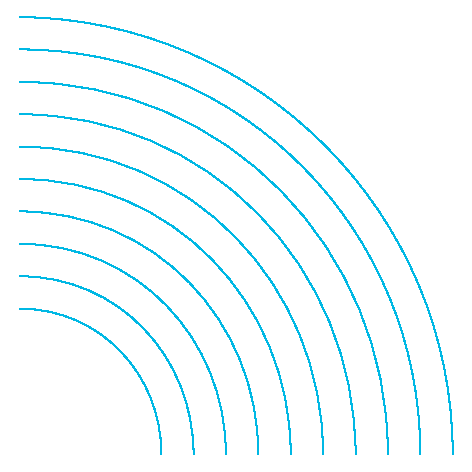
\includegraphics[width=.15\paperwidth,height=.15\paperwidth]{EETtemplateFiles/img/Simbolo_ESCOLA.pdf}\\
  
\includegraphics[width=.15\paperwidth,trim={.4cm .5cm .4cm 2.25cm},clip]{EETtemplateFiles/img/Logotipo_ESCOLA.pdf}
  \vspace*{-11pt}%
}

% MATH SYMBOLS

\newcommand{\field}[1]{\mathbb{#1}}

\DeclareMathOperator{\atan}{atan}
\DeclareMathOperator{\acos}{acos}
\DeclareMathOperator{\asin}{asin}

% \newcommand{\mb}[1]{\mathbf{#1}}


\newcommand{\Hb}{\mathbf{H}}
\newcommand{\Sb}{\mathbf{\boldsymbol{\Sigma}}}
\newcommand{\Sm}{\mathbf{S}}
\newcommand{\U}{\mathbf{U}}
\newcommand{\F}{\mathbf{F}}
\newcommand{\V}{\mathbf{V}}
\newcommand{\A}{\mathbf{A}}
\newcommand{\B}{\mathbf{B}}
\newcommand{\Cb}{\mathbf{C}}
\newcommand{\D}{\mathbf{D}}
% \newcommand{\E}{\mathbf{E}}
\newcommand{\Gb}{\mathbf{G}}
\newcommand{\T}{\mathbf{T}}
\newcommand{\I}{\mathbf{I}}
\newcommand{\Y}{\mathbf{Y}}
\newcommand{\M}{\mathbf{M}}
\newcommand{\N}{\mathbf{N}}
\newcommand{\W}{\mathbf{W}}
\newcommand{\Z}{\mathbf{Z}}
\newcommand{\R}{\mathbf{R}}
\newcommand{\K}{\mathbf{K}}
\newcommand{\X}{\mathbf{X}}
\newcommand{\Pb}{\mathbf{P}}
\newcommand{\Lb}{\mathbf{L}}
\newcommand{\Phib}{\mathbf{\boldsymbol{\Phi}}}
\newcommand{\Upsb}{\mathbf{\boldsymbol{\Upsilon}}}
\newcommand{\Delb}{\mathbf{\boldsymbol{\Delta}}}
\newcommand{\Xib}{\mathbf{\boldsymbol{\Xi}}}
\newcommand{\Q}{\mathbf{Q}}
% \newcommand{\D}{\mathbf{D}}
\newcommand{\one}{\mathbf{1}}
\newcommand{\zero}{\mathbf{0}}
\newcommand{\Rm}{\mathbf{R^{-1}}}
\newcommand{\LL}{\mathbf{\boldsymbol{\Lambda}}}
\newcommand{\J}{\mathbf{J}}

\newcommand{\ab}{\mathbf{a}}
\newcommand{\bb}{\mathbf{b}}
\newcommand{\cc}{\mathbf{c}}
\newcommand{\dd}{\mathbf{d}}
\newcommand{\e}{\mathbf{e}}
\newcommand{\f}{\mathbf{f}}
\newcommand{\g}{\mathbf{g}}
\newcommand{\h}{\mathbf{h}}
\newcommand{\m}{\mathbf{m}}
\newcommand{\n}{\mathbf{n}}
\newcommand{\pp}{\mathbf{p}}
\newcommand{\q}{\mathbf{q}}
\newcommand{\rr}{\mathbf{r}}
\newcommand{\s}{\mathbf{s}}
\newcommand{\uu}{\mathbf{u}}
\newcommand{\vv}{\mathbf{v}}
\newcommand{\w}{\mathbf{w}}
\newcommand{\x}{\mathbf{x}}
\newcommand{\y}{\mathbf{y}}
\newcommand{\z}{\mathbf{z}}
\newcommand{\al}{\mathbf{\boldsymbol{\alpha}}}
\newcommand{\vmu}{\mathbf{\boldsymbol{\mu}}}
\newcommand{\vlambda}{\mathbf{\boldsymbol{\lambda}}}
\newcommand{\vphi}{\mathbf{\boldsymbol{\phi}}}
\newcommand{\vrho}{\mathbf{\boldsymbol{\rho}}}
\newcommand{\vups}{\mathbf{\boldsymbol{\upsilon}}}

\newcommand{\rank}{\textnormal{rank}}
% \newcommand{\trace}{\textnormal{trace}}
\newcommand{\exptr}{\textnormal{exptr}}
\newcommand{\tr}{\textnormal{tr}}
\newcommand{\vstack}{\textnormal{vec}}
\newcommand{\diag}{\textnormal{diag}}
%  |x>
\newcommand{\ket}[1]{\left\vert#1\right\rangle}
%  <x|
\newcommand{\bra}[1]{\left\langle#1\right\vert}
%  <x|y>
\newcommand{\braket}[2]{\left< #1 \vphantom{#2}\,
                        \right\vert\left.\!\vphantom{#1} #2 \right>}
%  <x|a|y>
\newcommand{\sandwich}[3]{\left< #1 \vphantom{#2 #3} \right|
                          #2 \min\left(\vphantom{#1 #2} #3 \right>}

\newcommand{\pd}[2]{\frac{\partial #1}{\partial #2}}
%  d/dt
\newcommand{\ddt}{\frac{d}{dt}}
%  D/Dx
\newcommand{\pdd}[1]{\frac{\partial}{\partial#1}}
%  |x|
\newcommand{\abs}[1]{\left\vert#1\right\vert}
%  k_{x}
\newcommand{\kv}[1]{\mathbf{k}_{#1}}
%  \textnormal{E}_{domain of integration}{variable}
\newcommand{\Ex}[2]{{\mathbb{E}_{#1}\left[#2\right]}}
\newcommand{\CEx}[3]{{\mathbb{E}_{#1}\left[#2|#3\right]}}
\newcommand{\CInf}[3]{{\textnormal{I}\left(#1;#2|#3\right)}}
\newcommand{\Inf}[2]{{\textnormal{I}\left(#1;#2\right)}}
\newcommand{\CEnt}[2]{{\textnormal{H}\left(#1|#2\right)}}
\newcommand{\Ent}[1]{{\textnormal{H}\left(#1\right)}}
\newcommand{\dCEnt}[2]{{\textnormal{h}\left(#1|#2\right)}}
\newcommand{\dEnt}[1]{{\textnormal{h}\left(#1\right)}}

\newcommand{\cmark}{\ding{51}}%
\newcommand{\xmark}{\ding{55}}%
\newcommand\Tau{\mathcal{T}}
%Figure and format fixes


\renewcommand{\figurename}{Fig.}
\newcommand{\PESrule}{\noindent\rule{.57\columnwidth}{0.1mm}}

% A command to make itemized table contents

%theroem environments
% If using amsthm package, we need to delete these theorems before giving them our own definition. does not work for theorem
% \let\theorem\relax
\let\definition\relax
\let\lemma\relax
\let\corollary\relax
\let\example\relax
%
% \newtheorem{theorem}{Theorem}
\newtheorem{definition}{Definition}
\newtheorem{lemma}{Lemma}
\newtheorem{corollary}{Corollary}
\newtheorem{conjecture}{Conjecture}
\newtheorem{example}{Example}
\theoremstyle{plain}
\newtheorem{remark}{Remark}
\newtheorem{proposition}{Proposition}
   \newtheorem{homework}{Homework}

%Colors
   \definecolor{blueH3}{rgb}{0,.5,1}
   \definecolor{blueH2}{rgb}{0,0.25,0.75}
   \definecolor{blueH1}{rgb}{0,0,0.5}   
   \definecolor{grayOldText}{rgb}{.5,.5,.5}
   \definecolor{VCobalt}{HTML}{005682}
   \definecolor{TZTeal}{HTML}{008080}
   \definecolor{TZTealfaded}{HTML}{F0FFFF}
   \definecolor{KYJade}{HTML}{008151}
   \definecolor{ARust}{HTML}{a10000}
   \definecolor{FFucsia}{HTML}{7000c3}   
   \definecolor{TAMustard}{HTML}{a1a100}
   \definecolor{Tangerine}{HTML}{d45500}
   
   %%%%%%%%%%%%%%%%%%%%%%%%%%%%%%%%%%%%%%%%%%%%%%%%%%%%%%%%%%%%%%%%%
%% The following definitions are to extend the LaTeX algorithmic 
%% package with SWITCH statements and one-line structures.
%% The extension is by 
%%   Prof. Farn Wang 
%%   Dept. of Electrical Engineering, 
%%   National Taiwan University. 
%% 
\newcommand{\SWITCH}[1]{\STATE \textbf{switch} (#1)}
\newcommand{\ENDSWITCH}{\STATE \textbf{end switch}}
\newcommand{\CASE}[1]{\STATE \textbf{case} #1\textbf{:} \begin{ALC@g}}
\newcommand{\ENDCASE}{\end{ALC@g}}
\newcommand{\CASELINE}[1]{\STATE \textbf{case} #1\textbf{:} }
\newcommand{\DEFAULT}{\STATE \textbf{default:} \begin{ALC@g}}
\newcommand{\ENDDEFAULT}{\end{ALC@g}}
\newcommand{\DEFAULTLINE}[1]{\STATE \textbf{default:} }
%% 
%% End of the LaTeX algorithmic package extension.

\newcounter{MYtempeqncnt}


%%%%%%%%%%%%%%%%%%%%%%%%%%%%%%%%%%%%%%%
% Commands to recall text later
%%%%%%%%%%%%%%%%%%%%%%%%%%%%%%%%%%%%%%%
\makeatletter
\newcommand\remembertext[2]{% #1 is a key, #2 is the text
  \immediate\write\@auxout{\unexpanded{\global\long\@namedef{mytext@#1}{#2}}}%
  #2%
}
%
\newcommand\recalltext[1]{%
  \ifcsname mytext@#1\endcsname
    \@nameuse{mytext@#1}%
  \else
    ``??''
  \fi
}

%%%%%%%%%%%%%%%%%%%%%%%%%%%%%%%%%%%%%%%%%%%%%%%%%%%%%%%%%%%%%%%%%%%%%%%%%%%%%%%%%%
%%% Paolo Casari: macros for automating section titling and comment formatting %%%
%%%%%%%%%%%%%%%%%%%%%%%%%%%%%%%%%%%%%%%%%%%%%%%%%%%%%%%%%%%%%%%%%%%%%%%%%%%%%%%%%%
\newcounter{myequationcnt}

\newcounter{rcnt}
\newcounter{ccnt}

\newcommand{\newreviewernopagebreak}[1]{\vspace{5em} \setcounter{ccnt}{0}\section*{\normalsize Comments of #1}\vspace{4mm}}

\newcommand{\ThisIsTheEditorNoPageBreak}{\setcounter{ccnt}{0}\section*{\Large Comments of the Editor}\vspace{3mm}}
\newcommand{\ThisIsTheEditor}{\clearpage \ThisIsTheEditorNoPageBreak}
\newcommand{\ThisIsANewReviewerNoPageBreak}[1]{\vspace{5em} \refstepcounter{rcnt}\label{r#1}\setcounter{ccnt}{0}\section*{\Large Comments of Reviewer \arabic{rcnt}}\vspace{3mm}}
\newcommand{\ThisIsANewReviewer}[1]{\clearpage\vspace{-5em} \ThisIsANewReviewerNoPageBreak{#1}}

\newcommand{\edcomment}[1]{
\begin{tcbremark}
\color{VCobalt}
    \refstepcounter{ccnt}\label{e\arabic{ccnt}}\noindent\textbf{\boldmath\emph{Comment E.\arabic{ccnt}:}} #1\vspace{0.2cm}
\end{tcbremark}
}
\newcommand{\refedcomment}[1]{E.\ref{e#1}}

\newcommand{\revcomment}[1]{
\begin{tcbremark}
\color{VCobalt}
\refstepcounter{ccnt}\label{r\arabic{rcnt}c\arabic{ccnt}}\noindent\textbf{\boldmath\emph{Comment \arabic{rcnt}.\arabic{ccnt}:}} #1\vspace{0.2cm}
\end{tcbremark}
}
\newcommand{\refrevcomment}[2]{\ref{r#1}.\ref{r#1c#2}}

% \newcommand{\ouranswer}[1]{\noindent\emph{Answer:} #1\vspace{0.6cm}}
% \newcommand{\citepap}[1]{\vspace{0.33cm}\begin{minipage}{0.05\textwidth} $\phantom{A}$  \end{minipage}\begin{minipage}{0.85\textwidth}\renewcommand{\baselinestretch}{1.15}\small \emph{#1} \end{minipage}\vspace{0.3cm}}

\newlength{\ansspace}
\addtolength{\ansspace}{0.6cm}
\newcommand{\ansbreak}{\vspace{\ansspace}}

\newlength{\stdleftskip}
\addtolength{\stdleftskip}{\leftskip}
\newlength{\stdrightskip}
\addtolength{\stdrightskip}{\rightskip}
\newlength{\citeskip}
\addtolength{\citeskip}{2em}
\newcommand{\oldbaselinestretch}{1.5}

\newcommand{\setcitepapskip}{%
    \leftskip\citeskip %
    \rightskip\citeskip %
    \renewcommand{\baselinestretch}{1.15}\small%
    \vspace{0.6em}%
    \noindent%
}

\newcommand{\resetLRmargins}{%
    \leftskip\stdleftskip %
    \rightskip\stdrightskip %
    \renewcommand{\baselinestretch}{\oldbaselinestretch}\normalsize %
    \vspace{0.6em}
}

\newcommand{\emans}{\emph{Answer:\ }}


%---------------
% LIMIAR
%---------------
%configuracion de opcions de beamer persoais, pero alleas ao estilo

% COMANDO QUE INTRODUCE UNHA DIAPOSITIVA CUN ÍNDICE NO QUE APARECEN VELADAS TÓDALAS SECCIÓNS MENOS A ACTUAL. ÚTIL PARA INTRODUCIR OS TÍPICOS ÍNDICES INTERMEDIOS.
\newcommand{\Inter}{\frame{\tableofcontents[currentsection]}}
\newcommand{\inter}{\frame{\tableofcontents[currentsection,currentsubsection]}}

% Pes de imaxe
\renewcommand{\figurename}{Fig.}
\addto\captionsenglish{\renewcommand{\figurename}{Fig.}}
\setbeamertemplate{caption}[numbered]

%ESTE PAQUETE PERMITE POÑER A BIBLIOGRAFIA AO PE DE PAXINA CON CONFIGURACIONS ESTETICAS PERSOAIS
% \usepackage[style=ieee,doi=false,isbn=false,url=true,backend=bibtex]{biblatex}
% \bibliography{./bibliografia.bib}
% \newrobustcmd*{\footfullcitenomark}{%
%   \AtNextCite{%
%     \let\thefootnote\relax 
%     \let\mkbibfootnote\mkbibfootnotetext
%     }%
%   \footfullcite}

%paquete para engadir notas de guion ao pdf
\usepackage{pgfpages}
% \setbeameroption{show only notes} 
% \setbeameroption{show notes}
% \setbeameroption{show notes on second screen=right}
% DATOS DO DOCUMENTO
\title{Advanced Communication Systems}
\subtitle{Part 2.1:\\ Multi-user Communications:\\ Multiple Access Channel}
\author[FGC]{Felipe G\'omez Cuba}
\institute[XX]{
\begin{columns}[T]
\begin{column}{9cm}\centering
Despacho 204\\
Titorías: Lun-Xov 15:00-16:30\\
(En caso de confinamento: videochamada a calquera horario acordado)\\
  \texttt{gomezcuba@gts.uvigo.es}\\
\end{column}
\end{columns}
}

\date{26 \& 28 October \& 2 November 2020 }

\begin{document}

% Diapositiva co título
%\frame[plain]{\titlepage}%the ``classic'' beamer cover pageç

\frame{\frametitle{\\}%generate top bar, but blank line as tittle
\titlepage
}%approximation to the ``GPSC ppt'' cover page, but with central beamer title

% \frame{\tableofcontents}
% \note[itemize]{%itemized notes are special ``note'' slides that beamer can append to the pdf or not, depending on a boolean toggle option
% \item Introduce yourself
% \item In this work we studied blablabla.
% }


\frame{\frametitle{Information Theory in One Page}
    \begin{definition}[Differential Entropy of random variable $X$]
    \begin{equation}
    h(X) =-\Ex{X}{\log(p(x))}=\int_{x\in\mathcal{X}}p(x)\log(\frac{1}{p(x)})
    \end{equation}
    \end{definition}
    \begin{definition}[\textbf{mutual information} between r.v.s $X$ and $Y$]
        $$\Inf{X}{Y}=\Ent{X}-\CEnt{X}{Y}=\int_x\int_yf(x,y)\log\left(\frac{f(x,y)}{f(x)f(y)}\right)$$
    \end{definition}
    \begin{theorem}[s]
    \begin{tabular}{c|c|c}
    Conditioning & Chain Rule & Capacity \\
    $\Ent{X}\geq\CEnt{X}{Y}$&$\Ent{X,Y}=\Ent{X}+\CEnt{Y}{X}$&$C=\sup_{f(x)} \Inf{X}{Y}$
    \end{tabular}
    \end{theorem}
}

\frame{\frametitle{AWGN MIMO Channel}
\begin{itemize}
 \item Discrete Equivalent Channel (DEC) $$\y=\Hb\x+\z$$
 \item Capacity vs different constraints
    \begin{itemize}
        \item Given a fixed covariance matrix $\Ex{}{\x\x^H}=\Sb_x$
            \begin{equation}
            \label{eq:CfixK}
            C(\Sb_x)=\log\det\left(\I+\frac{1}{\sigma_z^2}\Hb\Sb_x\Hb^H\right)
            \end{equation}
        \item Optimized $\Sb_x$ with CSIR (isotropic tx.)
            \begin{equation}
            \label{eq:Ccsir}
                C=\sup_{\Sb_x}\{C(\Sb_x)\}=\log\det\left(\I+\frac{P}{N_t\sigma_z^2}\Hb\Hb^H\right)
            \end{equation}
        \item Optimized $\Sb_x$ with CSIT (eigenvalue beamforming)
            \begin{equation}
            \label{eq:Ccsit}
                C=\sup_{\Sb_x|\Hb}\{C(\Sb_x)\}=\sum\log\left(1+\frac{P_i\lambda_i}{\sigma_z^2}\right)
            \end{equation}
    \end{itemize}
\end{itemize}
}


\frame[allowframebreaks]{\frametitle{Multiple Access Channel}   
        \begin{figure}
            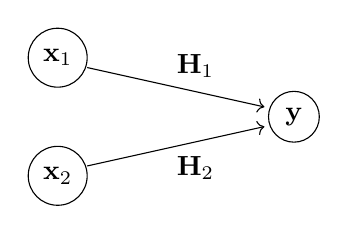
\begin{tikzpicture}[scale=.5]
                \draw [->] (.75,1.25) -- (5.25,.25);
                \draw [->] (.75,-1.25) -- (5.25,-.25);
                \node[draw,circle] at (0,1.5) {$\x_1$};
                \node[draw,circle] at (0,-1.5) {$\x_2$};
                \node[draw,circle] at (6,0) {$\y$};
                \node[anchor=south] at (3.5,.75) {$\Hb_1$};
                \node[anchor=north] at (3.5,-.75) {$\Hb_2$};
            \end{tikzpicture}
            \end{figure}


    \begin{itemize}
     \item Directed graph with $K$ transmitters and one receiver
     \begin{itemize}
        \item Each user $k$ encodes signal $\x_k$ \textit{independently}
        \item General case $Y \sim f(\y|\x_1,\x_2\dots,\x_k)$\\ \ \\
    \end{itemize}
    \item AWGN MAC channel
        $$\y = \sum_{k=1}^{K}\Hb_k\x_k+\z$$ 
     \item Example: \textit{Uplink} in a mobile cellular system\\ \ \\
     \item All devices may have one or multiple antennas\\ \ \\
     \item Each $\x_k$ is an independent message encoded with rate $R_k$
    \end{itemize}
    \begin{definition}[Rate Vector]
     $K-$ dimensional vector representing the $K$ rates by all users $\vec{R}=(R_1,R_2,\dots,R_K)$
    \end{definition}
    \begin{definition}[Capacity Region]
     $\mathcal{C}$ is the set of all rate vectors that can be achieved \textit{reliably} by all users
    \end{definition}
}
\frame{\frametitle{Outer Bound of Capacity Region}
    \begin{theorem}[Cut-Set Bound]
     The maximum flow across any cut-set in a graph cannot be greater than the sum of the capacities of the cut edges
    \end{theorem}    
    \begin{columns}
        \begin{column}{6cm}
        \begin{figure}
            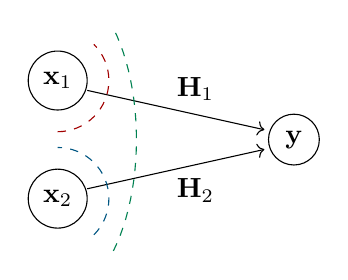
\begin{tikzpicture}[scale=.5]
                \draw [->] (.75,1.25) -- (5.25,.25);
                \draw [->] (.75,-1.25) -- (5.25,-.25);
                \node[draw,circle] at (0,1.5) {$\x_1$};
                \node[draw,circle] at (0,-1.5) {$\x_2$};
                \node[draw,circle] at (6,0) {$\y$};
                \node[anchor=south] at (3.5,.75) {$\Hb_1$};
                \node[anchor=north] at (3.5,-.75) {$\Hb_2$};
                 \onslide<1->{\draw [ARust,dashed,domain=-90:45] plot ({1.3*cos(\x)}, {1.5+1.3*sin(\x)});}
                 \onslide<2->{\draw [VCobalt,dashed,domain=-45:90] plot ({1.3*cos(\x)}, {-1.5+1.3*sin(\x)});}
                 \onslide<3->{\draw [KYJade,dashed,domain=-45:45] plot ({2*cos(\x)}, {4*sin(\x)});}
            \end{tikzpicture}
            \end{figure}
        \end{column}
        \begin{column}{6cm}
            \begin{figure}
            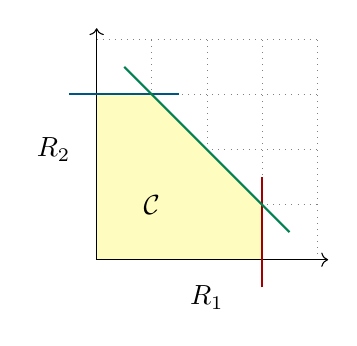
\begin{tikzpicture}[scale=.7]
                \draw[help lines,color=gray,dotted] (0,0) grid (4,4);
         \onslide<3->{\fill[color=yellow!25] (0,0) -- (3,0) -- (3,1) -- (1,3) -- (0,3) -- (0,0);}      
                \draw [->] (0,0) -- (0,4.2);
                \draw [->] (0,0) -- (4.2,0);
                \node [anchor=north] at (2,-0.3) {$R_1$}; 
                \node [anchor=east] at (-0.3,2) {$R_2$}; 
%                 \foreach \x in {0,1,...,4} { \node [anchor=north] at (\x,-0.3) {\tiny \x}; }
%                 \foreach \y in {0,1,...,4} { \node [anchor=east] at (-0.3,\y) {\tiny \y}; }          
         \onslide<1->{\draw[color=ARust,thick] (3,-.5) -- (3,1.5);}                
         \onslide<2->{\draw[color=VCobalt,thick] (-.5,3) -- (1.5,3);}                
         \onslide<3->{\draw[color=KYJade,thick] (.5,3.5) -- (3.5,.5);}
         \onslide<3->{\node at (1,1) {$\mathcal{C}$}; }
         
            \end{tikzpicture}
            \end{figure}
        \end{column}
    \end{columns}
\begin{equation}
  \mathcal{C}\subset \left\{
    \begin{array}{rl}
        \onslide<1->{
            \textcolor{ARust}{R_1}&\textcolor{ARust}{\leq \CInf{\x_1}{\y}{\Hb_1,\Hb_2\x_2}}\\
            }
         \onslide<2->{
            \textcolor{VCobalt}{ R_2}&\textcolor{VCobalt}{\leq \CInf{\x_2}{\y}{\Hb_1\x_1,\Hb_2}}\\
            }
         \onslide<3->{
            \textcolor{KYJade}{ R_1+R_2}&\textcolor{KYJade}{ \leq \CInf{\x_1,\x_2}{\y}{\Hb_1,\Hb_2}}
            }
    \end{array}
 \right\}
\end{equation}
}

\frame{\frametitle{MAC Capacity Region}
    \begin{itemize}
     \item Define a subset of users $\mathcal{S}\subset\{1,2,\dots K\}$\\ \ \\
     \item For \textit{any} subset, we can define a cut set bound
        $$\mathrm{CSB}(\mathcal{S})\triangleq \CInf{ \{\x_k\}_{k\in\mathcal{S}}}{\y}{\{\Hb_k\}_{k\in\mathcal{S}},\{\Hb_{k'}\x_{k'}\}_{k'\notin\mathcal{S}}}$$
    \end{itemize}
    \begin{theorem}[MAC Capacity Region]
        $\mathcal{C}$ is contained in the intersection of all cut-set bound constraints
        \begin{equation}
        \label{eq:macCreg}
         \mathcal{C}\subset \left\{\vec{R}:\forall \mathcal{S}\subset\{1\dots K\}\sum_{k\in\mathcal{S}} R_k\leq \mathrm{CSB}(\mathcal{S})
\right\}
        \end{equation}
    \end{theorem}
    \begin{remark}[Chain Rule]
%      \begin{enumerate}[A]
      $\CInf{\x_1,\x_2}{\y}{\Hb_1,\Hb_2} = \underset{\geq 0}{\underbrace{\CInf{\x_1}{\y}{\Hb_1,\Hb_2}}} + \CInf{\x_2}{\y}{\x_1,\Hb_1,\Hb_2}$
%       \item $\CInf{\x_1}{\y}{\Hb_1,\Hb_2} \geq 0$
%       \item A\&B $\to$ $\mathrm{CSB}(\mathcal{S}\cup \{k'\})\geq\mathrm{CSB}(\mathcal{S})$
%      \end{enumerate}
    \end{remark}
}

\frame[allowframebreaks]{\frametitle{AWGN MAC Capacity Region}
    \begin{itemize}
     \item Separate user rates limited by point-to-point link
        \begin{equation}
        \begin{split}
            R_k&\leq \sup_{f(\x_k)} \CInf{\x_k}{\y}{\Hb_k,\{\Hb_{k'}\x_{k'}\}_{k'\neq k}} \\
               &=\sup_{\Sb_{\x_k}}B\log\left|\I+\frac{1}{BN_o}\Hb_k\Sb_{\x_k}\Hb_k^H\right|          
        \end{split}
        \end{equation}
        
     \item Joint user rates limited by CSBs and chain rules
        \begin{equation*}
        \begin{split}
            R_1+R_2+\dots+R_K&\leq \sup_{f(\x_{tot})} \CInf{\x_{tot}}{\y}{\Hb_{tot}} \\
                         &= \sup_{f(\x_{tot})} \CInf{\x_{1}}{\y}{\Hb_{tot}}+\CInf{\x_{2}}{\y}{\Hb_{tot}|\x_1}+\CInf{\x_{3}}{\y}{\Hb_{tot},\x_1,\x_2} \dots 
        \end{split}
        \end{equation*}
     where $\x_{tot}=\left(\x_1^T|\dots|\x_K^T\right)^T$ and $\Hb_{tot}=\left(\Hb_1\dots\Hb_K\right)$
     \pagebreak
     \item Let's focus on single-antenna case for now, the expansion becomes   
        \begin{equation}\tiny
        \begin{split}
            R_1+\dots+R_K&\stackrel{SISO}{=}B\log\left(1+\frac{P_1|h_1|^2}{\sum_{k=2}^{K}P_k|h_k|^2+BN_o}\right)\\
            &\;\;\;+B\log\left(\tiny 1+\frac{P_2|h_2|^2}{\sum_{k=3}^{K}P_k|h_k|^2+BN_o}\right)\\
            &\;\;\;+\dots\\
            &\;\;\;+B\log\left(\tiny 1+\frac{P_K|h_K|^2}{BN_o}\right)
        \end{split}
        \end{equation}
        \begin{definition}[Signal To Interference Noise Ratio of user $k$]
        \begin{equation}
         \gamma_k\triangleq = \frac{P_k|h_k|^2}{\sum_{k'=k+1}^{K}P_{k'}|h_{k'}|^2 + BN_o}
        \end{equation}
    \end{definition}
        
\pagebreak
\item For the 2-user case $\mathcal{C}$ is a pentagon
    \begin{columns}
        \begin{column}{5cm}
            \begin{figure}
            \begin{tikzpicture}[scale=.7]
                \draw[help lines,color=gray,dotted] (0,0) grid (4,4);
                \draw [->] (0,0) -- (0,4.2);
                \draw [->] (0,0) -- (4.2,0);
                \node [anchor=north] at (2,-0.3) {$R_1$}; 
                \node [anchor=east] at (-0.3,2) {$R_2$}; 
%                 \foreach \x in {0,1,...,4} { \node [anchor=north] at (\x,-0.3) {\tiny \x}; }
%                 \foreach \y in {0,1,...,4} { \node [anchor=east] at (-0.3,\y) {\tiny \y}; }                
         \draw[color=ARust,thick] (3,0) -- (3,1);
         \draw[color=VCobalt,thick] (0,3) -- (1,3);                
         \draw[color=KYJade,thick] (1,3) -- (3,1);
         \draw[color=black,thin] (3,1) circle (.1);
         \fill[color=white,thin] (3,1) circle (.1);
         \node[anchor=south] at (3,1) {A};
         \draw[color=black,thin] (1,3) circle (.1);
         \fill[color=white,thin] (1,3) circle (.1);
         \node[anchor=south] at (1,3) {B};
            \end{tikzpicture}
            \end{figure}
        \end{column}
        \begin{column}{6.5cm}
        \begin{itemize}
         \item Point A:
          \begin{equation}
            \begin{array}{rl}
                    R_1&= B\log\left(1+\frac{P_1|h_1|^2}{BN_o}\right)\\
                    R_2&= B\log\left(1+\frac{P_2|h_2|^2}{P_1|h_1|^2+BN_o}\right)\\
            \end{array}
          \end{equation}
         \item Point B:
          \begin{equation}
            \begin{array}{rl}
                    R_1&= B\log\left(1+\frac{P_1|h_1|^2}{P_2|h_2|^2+BN_o}\right)\\
                    R_2&= B\log\left(1+\frac{P_2|h_2|^2}{BN_o}\right)\\
            \end{array}
          \end{equation}
        \end{itemize}       
        \end{column}
    \end{columns}
    \item For the $N$-user case $\mathcal{C}$ is a $N$-dimensional polyhedron
        \begin{itemize}
            \item There are $N!$ ``corner points''
            \item Each corresponds to a permutation of the list $\{1,2,\dots K\}$.
        \end{itemize}
        
        
\pagebreak
     \item Calculating the chain rule terms for MIMO
\begin{definition}[Markov Chain $X\to Y\to Z$]
    If random variables $X,Y,Z$ satisfy $f(Z|Y,X)=f(Z|Y)$ then $\Inf{X}{Z}\leq\Inf{X}{Y}$
    
    ``$Z$ depends on $X$ only through $X$''
\end{definition}

\begin{theorem}
When all inputs are Gaussian $\CInf{\x_k}{\y}{\Hb_k,\{\Hb_{k'}\x_{k'}\}_{k'=1}^{k-1}}=$
    $$        \log\left|\I+\left(\sum_{k'=k+1}^{K}\Hb_{k'}\Sb_{\x_{k'}}\Hb_{k'}^H+\Sb_{\z}\right)^{-1}\Hb_{k}\Sb_{\x_{k}}\Hb_{k}^H\right|$$
\end{theorem}
\pagebreak
\vspace{-.5in}
\begin{proof}
\begin{itemize}
 \item Compute $\rr_k = \y-\sum_{k'=1}^{u-1}\Hb_{k'}\x_{k'}$\\ \ \\
 \item Double Markov Chain $\x_k \leftrightarrow \y|\{\Hb_{k'}\x_{k'}\}_{k'=1}^{u-1} \leftrightarrow \rr_k$
    $$\CInf{\x_k}{\y}{\Hb_k,\{\Hb_{k'}\x_{k'}\}_{k'=1}^{u-1}}=\CInf{\x_k}{\rr_k}{\Hb_k}$$
 \item $f(\rr_k)\sim \mathcal{CN}(0,\sum_{\textcolor{ARust}{k'=k}}^{K}\Hb_{k'}\Sb_{\x_{k'}}\Hb_{k'}^H+\Sb_\z)$\\ \ \\
 \item $f(\rr_k|\x_k,\Hb_k)\sim \mathcal{CN}(\Hb_k\x_k,\sum_{\textcolor{ARust}{k'=k+1}}^{K}\Hb_{k'}\Sb_{\x_{k'}}\Hb_{k'}^H+\Sb_\z)$\\ \ \\
 \item Gaussian $f(\x)=\pi^{-N}\det(\Sb)^{-1}e^{-(\x-\vec\mu)^H\Sb^{-1}(\x-\vec\mu)}$\\ \ \\
 \item $\det(\A)/\det(\B)=\det(\B^{-1}\A)$
\end{itemize} 
\end{proof}
    \end{itemize}
    
}

\frame{\frametitle{Inner Bound of Capacity Region}
\vspace{-.1in}
\begin{theorem}[Capacity Region is Convex]
 If two methods achieve rate vectors $\vec{R}_A$ and $\vec{R}_B$, any linear combination can by achieved by time-sharing.
% \vspace{-.1in}
 $$\vec{R}_A\in \mathcal{C}\textnormal{ and }\vec{R}_B\in \mathcal{C} \Rightarrow \alpha\vec{R}_A+(1-\alpha)\vec{R}_B \in \mathcal{C}\;\forall\alpha\in[0,1]$$
\end{theorem}
\vspace{-.25in}
    \begin{columns}
        \begin{column}{4cm}
            \begin{figure}
            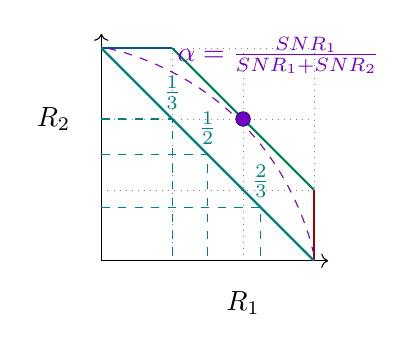
\begin{tikzpicture}[scale=.9]
                \draw[help lines,color=gray,dotted] (0,0) grid (3,3);
                \draw [->] (0,0) -- (0,3.2);
                \draw [->] (0,0) -- (3.2,0);
                \node [anchor=north] at (2,-0.3) {$R_1$}; 
                \node [anchor=east] at (-0.3,2) {$R_2$}; 
%                 \foreach \x in {0,1,...,4} { \node [anchor=north] at (\x,-0.3) {\tiny \x}; }
%                 \foreach \y in {0,1,...,4} { \node [anchor=east] at (-0.3,\y) {\tiny \y}; }                
         \draw[color=ARust,thick] (3,0) -- (3,1);
         \draw[color=VCobalt,thick] (0,3) -- (1,3);                         
         \draw[color=KYJade,thick] (1,3) -- (3,1);             
         \onslide<1-1>{
         \draw[color=TZTeal,dashed] (0,2) -- (1,2) -- (1,0); 
         \node[color=TZTeal,anchor=south] at (1,2) {$\tiny\frac{1}{3}$};
         \draw[color=TZTeal,dashed] (0,1.5) -- (1.5,1.5) -- (1.5,0);
         \node[color=TZTeal,anchor=south] at (1.5,1.5) {$\tiny\frac{1}{2}$};
         \draw[color=TZTeal,dashed] (0,3/4) -- (9/4,3/4) -- (9/4,0); 
         \node[color=TZTeal,anchor=south] at (9/4,3/4) {$\tiny\frac{2}{3}$};
         }         
         \draw[color=TZTeal,thick] (0,3) -- (3,0);            
         \onslide<2->{
            \draw [FFucsia,dashed,domain=1:99] plot ({0.01*\x*ln(1+7.1*100/\x)/ln(2)}, {0.01*(100-\x)*ln(1+7.1*100/(100-\x))/ln(2)});
            \draw[thin] (2,2) circle (.1);
            \fill[color=FFucsia,thin] (2,2) circle (.1);
            \node[anchor=south,color=FFucsia] at (2.5,2.5) {$\tiny \alpha=\frac{SNR_1}{SNR_1+SNR_2}$};
         }
            \end{tikzpicture}
            \end{figure}     
         \vspace{-.2in}
        \begin{itemize}
            \item \textcolor{TZTeal}{$\gamma_k^{TDMA}$ = SNR$^{SISO}$}
          \onslide<2->{
            \item \textcolor{FFucsia}{$\gamma_k^{FDMA}$ > SNR$^{SISO}$}
            }
        \end{itemize}
        \end{column}
        \begin{column}{8cm}
        \begin{itemize}
         \item \textcolor{TZTeal}{Time Division Multiple Access (TDMA) $\alpha$
          \begin{equation}
            \begin{array}{rl}
                    R_1&= \alpha B\log\left(1+\frac{P_1|h_1|^2}{BN_o}\right)\\
                    R_2&= (1-\alpha) B\log\left(1+\frac{P_2|h_2|^2}{BN_o}\right)\\
            \end{array}
          \end{equation}}
         \vspace{-.2in}
          \onslide<2->{
         \item \textcolor{FFucsia}{Freq. Division Multiple Access (FDMA) $\alpha$
          \begin{equation}
            \begin{array}{rl}
                    R_1&= \alpha B\log\left(1+\frac{P_1|h_1|^2}{\alpha BN_o}\right)\\
                    R_2&= (1-\alpha) B\log\left(1+\frac{P_2|h_2|^2}{(1-\alpha) BN_o}\right)\\
            \end{array}
          \end{equation}}}
        \end{itemize}       
        \end{column}
    \end{columns}
}


\frame[allowframebreaks]{\frametitle{Achieving Capacity Region}
    \begin{definition}
     \textbf{Non-Orthogonal Multiple Access (NOMA)}, or ``multiplexing in the power domain'' are industry names for practical applications of the capacity-achieving schemes in the MAC channel.
    \end{definition}
    
    \begin{itemize}
     \item Successive Interference Cancelling (SIC)
        \begin{itemize}
        \item Inspired by the chain rule\\ \ \\
        \item Dimilar to DF in MIMO single-user channel\\ \ \\
        \item Select a permutation of the list of users $(\pi(1),\pi(2)\dots\pi(U))$\\ \ \\
        \item Decode $x_{\pi(1)}$, substract $y-h_{1}x_{\pi(1)}$, and so on...
        \end{itemize}

    \end{itemize}

    \begin{columns}
        \begin{column}{5cm}
            \begin{figure}
            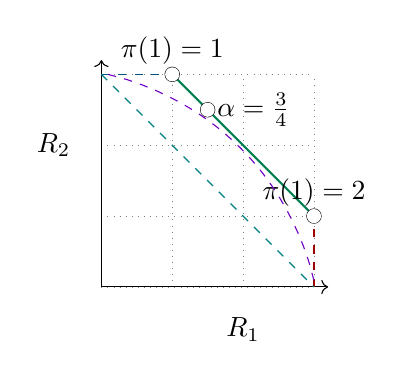
\begin{tikzpicture}[scale=.9]
                \draw[help lines,color=gray,dotted] (0,0) grid (3,3);
                \draw [->] (0,0) -- (0,3.2);
                \draw [->] (0,0) -- (3.2,0);
                \node [anchor=north] at (2,-0.3) {$R_1$}; 
                \node [anchor=east] at (-0.3,2) {$R_2$}; 
%                 \foreach \x in {0,1,...,4} { \node [anchor=north] at (\x,-0.3) {\tiny \x}; }
%                 \foreach \y in {0,1,...,4} { \node [anchor=east] at (-0.3,\y) {\tiny \y}; }                
         \draw[color=ARust,dashed] (3,0) -- (3,1);
         \draw[color=VCobalt,dashed] (0,3) -- (1,3);                         
         \draw[color=KYJade,thick] (1,3) -- (3,1);    
         \draw[color=black,thin] (3,1) circle (.1);
         \fill[color=white,thin] (3,1) circle (.1);
         \node[anchor=south] at (3,1) {$\pi(1)=2$};
         \draw[color=black,thin] (1,3) circle (.1);
         \fill[color=white,thin] (1,3) circle (.1);
         \node[anchor=south] at (1,3) {$\pi(1)=1$};
         \draw[color=black,thin] (1.5,2.5) circle (.1);
         \fill[color=white,thin] (1.5,2.5) circle (.1);
         \node[anchor=west] at (1.5,2.5) {$\alpha=\frac{3}{4}$};
         \draw[color=TZTeal,dashed] (0,3) -- (3,0);            
        \draw [FFucsia,dashed,domain=1:99] plot ({0.01*\x*ln(1+7.1*100/\x)/ln(2)}, {0.01*(100-\x)*ln(1+7.1*100/(100-\x))/ln(2)});
            \end{tikzpicture}
            \end{figure}
        \end{column}
        \begin{column}{7cm}
    \begin{itemize}
     \item \textcolor{KYJade}{\textbf{Pareto Front}} $\subset$ border of $\mathcal{C}$\\ \ \\
     \item Corner Points: 
        \begin{itemize}
            \item Achieved using SIC
            \item One for each different decoding order permutation $\pi(1),\pi(2)\dots$\\ \ \\
        \end{itemize}
     \item Edge Lines:
        \begin{itemize}
            \item Linear combination of corners
            \item Achievable using time-multiplexing\\ \ \\
        \end{itemize}
    \end{itemize}
        \end{column}
    \end{columns}
    
    
    \begin{remark}
     SIC with $\Q\R$ decomposition (as in 1 user MIMO) does not help in multi-user xISO: for a single-row matrix $\Hb_{tot}=\left(h_1,\dots h_K\right)$, we get $\Q=1$ and $\R=\Hb_{tot}$
    \end{remark}
}

\frame{\frametitle{Homework \#5: Rate Splitting}
%     \begin{homework}
        Sometimes time-multiplexing is inconvenient. Consider a system where User 2 divides their available power in two virtual users:
        \begin{enumerate}
         \item Virtual user 2A transmits with power $\delta P_2$
         \item Actual user 1 transmits with power $P_1$
         \item Virtual user 2B transmits with power $(1-\delta) P_2$
        \end{enumerate}
      \textbf{Show how a successive decoding strategy 2A,1, 2B can be used to obtain any point in the maximum sum-rate boundary (segment AB) by varying $\delta$ between $0$ and $1$.}
%     \end{homework}
}


\frame[allowframebreaks]{\frametitle{Code Division Multiple Access (3G)}
    \begin{itemize}
     \item Each $k$ has a ``spreading code'' $c_k[.]$ of length $L$
     \item Data symbol sequence $s_k[.]$ with sampling rate $\times 1/L$
     \item Transmitted signal has bandwidth $\times L$ data symbol rate
        $$x_k[n]=s_k[\lfloor n/L \rfloor]c[n \mod L]$$
        \begin{figure}
            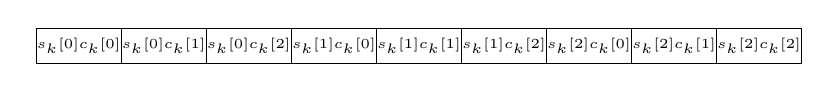
\begin{tikzpicture}[scale=.9]
              \foreach \x in {0,1,...,2} { 
                \foreach \y in {0,1,...,2} { 
                    \draw (1.2*\x+3.6*\y,0) rectangle (1.2+1.2*\x+3.6*\y,.5);
                    \node [anchor=center] at (1.2*\x+3.6*\y+.6,.25) {\tiny $s_k[\y]c_k[\x]$}; 
                    }
                }
            \end{tikzpicture}
        \end{figure}
    \item Orthogonal ($\sum_{\ell=0}^{L}c_k[\ell]^*c_{k'}[\ell]=0$) similar to FDMA\\ \ \\
    \item Non-orthogonal ($\sum_{\ell=0}^{L}c_k[\ell]^*c_{k'}[\ell]=\frac{1}{L}$): $\gamma_k=\frac{P_k}{N_o\frac{B}{L}+\sum_{k'\neq u}P_{k'}/L}$\\ \ \\
    \item Non-orthogonal + SIC: still worse than rate splitting
        $$B/L\log\left(1+\frac{LP_1}{N_oB+P_2}\right)\leq B\log\left(1+\frac{P_1}{N_oB+P_2}\right)$$
    \end{itemize}

}


\frame[allowframebreaks]{\frametitle{\small Orthogonal Frequency Division Multiple Access  (4G)}
    \begin{itemize}
        \item In general for each OFDM symbol $n$ and subcarrer $k$
            $$\y[n,k]=\sum_{k}\Hb_k\x_k[n,k]+\z[n,k]$$
        \item Assign to each user $k$ a different subset $\mathcal{A}(k)$ of the grid $(n,k)\in\{1\dots N\}\times\{1\dots K\}$    
            \begin{figure}
            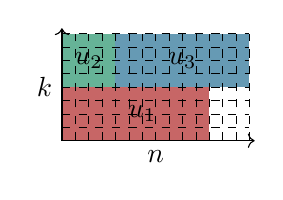
\begin{tikzpicture}[scale=.17]
                \fill[color=VCobalt!60] (4,4) rectangle (14,8);
                \fill[color=KYJade!60] (4,4) rectangle (0,8);
                \fill[color=ARust!60] (0,0) rectangle (11,4);
                \draw[help lines,color=black,dashed] (0,0) grid (14,8);   
                \draw [->] (0,0) -- (0,8.4);
                \draw [->] (0,0) -- (14.4,0);
                \node [anchor=center] at (6,2) {$u_1$};
                \node [anchor=center] at (2,6) {$u_2$};
                \node [anchor=center] at (9,6) {$u_3$};
                \node [anchor=north] at (7,0) {$n$};
                \node [anchor=east] at (0,4) {$k$};         
            \end{tikzpicture}
            \end{figure}
         \item Time \textbf{and} frequency orthogonal channel divisions
             $$\y[n,k]=\Hb_{\mathcal{A}^{-1}(n,k)}\x_{\mathcal{A}^{-1}(n,k)}[n,k]+\z[n,k]$$        
         \item Hybrid method (interference user groups): $\mathcal{A}(k)\cap\mathcal{A}(k')\neq \emptyset$
    \end{itemize}
}


\frame[allowframebreaks]{\frametitle{Optimal Multi-user Detection}

    \begin{definition}
     An decoding error for the message of user $k$ occurs with probability $P(\hat{\x}_k\neq\x_k)$. Thus the \textit{system} error probability is
     \begin{equation}
      \begin{split}
       P(error)&=1-\prod_{k=1}^{K}(1-P(\hat{\x}_k\neq\x_k))\\
        &=P(\hat{\x}_1\neq\x_1)+P(\hat{\x}_2\neq\x_2\&\hat{\x}_1 = \x_1)\dots
      \end{split}
     \end{equation}
    \end{definition}
    
    \begin{theorem}
     For Orthogonal suboptimal schemes (TDMA,FDMA) the single-user ML detector is optimal. (Can you think why?)
    \end{theorem}
    
    \begin{itemize}
     \item We focus on non-orthogonal MUD case
    \end{itemize}

    \pagebreak
        
     $$\y= \sum_{k=1}^{K}\Hb_k\x_k+\z=\Hb_{tot}\x_{tot}+\z$$ 
     \begin{tabular}{llll}
%       Rec. & \textcolor{VCobalt}{\Large \ding{46}} & \textcolor{KYJade}{\Large \cmark} & \textcolor{ARust}{\Large \xmark} \\ \hline
      Sphere Dec. & $\displaystyle \min_{\mathcal{C}_1\times \mathcal{C}_2\times\dots}\|\y-\Hb_{tot}\x_{tot}\|^2$ & \textcolor{KYJade}{\Large \cmark} Fast ML & \textcolor{ARust}{\Large \xmark} Still NP\\
      &&& \textcolor{ARust}{\Large \xmark} Different $P_k$, $\mathcal{C}_k$... \\\hline
      Linear & $\rr=\W^H\y$ & \textcolor{KYJade}{\Large \cmark} MF & \textcolor{ARust}{\Large \xmark} Suboptimal $\gamma_k$ \\
      && \textcolor{KYJade}{\Large \cmark} ZF & \textcolor{ARust}{\Large \xmark} Symbol-by-symbol \\
      && \textcolor{KYJade}{\Large \cmark} MMSE &  \\ \hline
      DF & $\displaystyle \w_i^H\h_i x_i+\sum_{i'>i} \w_i^H\h_{i'}x_{i'}+z_i$ & \textcolor{KYJade}{\Large \cmark} SIC & \textcolor{ARust}{\Large \xmark} Permutations\\
      &&& \textcolor{ARust}{\Large \xmark} Error propagation \\ \hline
      IDD & $\displaystyle y_i = \w_i^H\h_i x_i + \xi_i + z_i$ &  \textcolor{KYJade}{\Large \cmark} $\mathrm{Var}^{(n)}(\xi_i)$ & \textcolor{ARust}{\Large \xmark} Req. FEC  \\
      
     \end{tabular}
    
}

\frame[allowframebreaks]{\frametitle{Linear Multi-user Detection}
    
    \begin{itemize}
     \item Linear filter design $\rr=\W^H\y$ 
     \begin{itemize}     
      \item Each row is a single-user combiner
      $$r_k=\w_k^H\y=\w_k^H\h_kx_k+\underset{\textnormal{treat as noise}}{\underbrace{\sum_{k'\neq k} \w_k^H\h_{k'} x_{k'}}} + \w_k^H\z$$
      \item Scalar decisor $\hat{x}_k=\mathcal{Q}_{\mathcal{C}_k}(r_k)$
      \item Very hard to take into account constellations $\mathcal{C}_k$
     \end{itemize}
%            \begin{theorem}
%        The worst noise of a give variance is Gaussian.
%       \end{theorem}
      \item Multi-objective optimizations on achievable rate region
      $$ \{\dot R_k(\gamma_k) \forall k\} \textnormal{ where } \gamma_k = \frac{|\w_k^H\h_k|^2P_k}{\sum_{k'\neq k}|\w_k^H\h_{k'}|^2P_{k'}+|\w_k|^2\sigma_z^2}$$      
           \begin{definition}[Achievable Rate]
    $\dot R(\gamma_k) = \log_2(1+\gamma_k) \equiv$ $C$ of a virtual AWGN channel with SNR = $\gamma_k$
%     \begin{equation}
%         \label{eq:achrate}
%         \dot R(\gamma) = \log_2(1+\gamma)
%     \end{equation}
    \end{definition}
     \pagebreak

     \item Known single-user filters:
     \begin{tabular}{l|l|l}
     MF & ZF & MMSE \\
     \textcolor{KYJade}{\Large \xmark} max SNR & \textcolor{KYJade}{\Large \cmark} no interference & \textcolor{KYJade}{\Large \cmark} max SINR \\
     \textcolor{ARust}{\Large \xmark} interference & \textcolor{ARust}{\Large \xmark} $\uparrow$ noise & \textcolor{KYJade}{\Large \cmark} max sum rate $\displaystyle \sum \dot R(\gamma_k)$\\    
     \end{tabular}
        \begin{theorem}[Matrix Inversion Lemma]
       $$\W_{MMSE}=\left(\Hb^H\Hb+\sigma^2\I\right)^{-1}\Hb^H=\Hb^H\left(\Hb\Hb^H+\sigma^2\I\right)^{-1}\to \w_k^H=\h_k^H\left(\Hb\Hb^H+\sigma^2\I\right)^{-1}$$
      \end{theorem}
     \item Specific multi-user optimization (choose a point in Pareto Front)
        \begin{itemize}
            \item Max worst user (maximin) $\displaystyle \max_{\W}\min_{k}\dot R_k(\gamma_k)$\\ \ \\
            \item Weighted linear combination $\displaystyle \max_{\W}\sum_{k} C_k R_k(\gamma_k)$
        \end{itemize}     
     \end{itemize}
     
     \pagebreak
     \begin{theorem}[Jensen's inequality]
      For any convex (concave) function $\phi(x)$ and random variable $X$, $\Ex{X}{\phi(x)}\geq(\leq){\phi(\Ex{X}{x})}$
     \end{theorem}
     
     \begin{theorem}[MUD with Heterogeneous Users]
      $$\sum_{k}\log(1+\gamma)\leq K\log(1+\overline\gamma),$$
     \end{theorem}
     \begin{itemize}
      \item Maximum achievable sum rate when all receivers have equal received power
      \item MAC channels with different transmit power, pathloss etc. are inherently worse
     \end{itemize}
}




\frame[allowframebreaks]{\frametitle{Slow Fading MAC Channel Outage}
\begin{columns}
 \begin{column}{7cm}
\begin{itemize}
  \item Recall single-user:
  \begin{itemize}
  \item Coh. time $T_c$ $\gg$ codeword $T_s L_{s}$
  \item $C_{out}\triangleq \sup \{R \textnormal{ s.t. }  F_{I}(R)\leq P_o\}$\\ \ \\
\end{itemize}
  \item $K$ random channels $f(\Hb_1,\dots,\Hb_K)$\\ \ \\
  \item Random rate region $\mathcal{C}_{\Hb}$ vs $\Hb$ \eqref{eq:macCreg}\\ \ \\
\end{itemize}
\begin{definition}[Outage Capacity \textbf{Region}]
  $$\mathcal{C}_{out}\triangleq \bigcup \{\vec{R} :  P\left(\vec{R}\notin\mathcal{C}_{\Hb}\right)\leq P_o\}$$
\end{definition}  
 \end{column}
 \begin{column}{5cm}
 $$\vec{R}\in \mathcal{C}_2\&\mathcal{C}_3\&\mathcal{C}_4\; \notin \mathcal{C}_1,\mathcal{C}_5$$
    \begin{figure}
            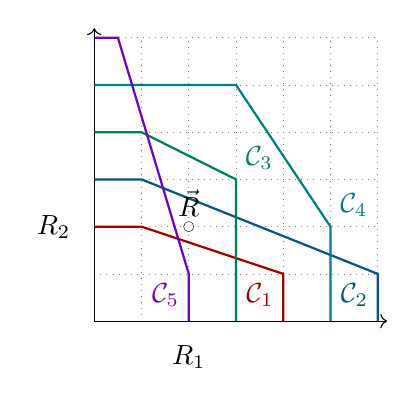
\begin{tikzpicture}[scale=.6]
                \draw[help lines,color=gray,dotted] (0,0) grid (6,6);
                \draw [->] (0,0) -- (0,6.2);
                \draw [->] (0,0) -- (6.2,0);
                \node [anchor=north] at (2,-0.3) {$R_1$}; 
                \node [anchor=east] at (-0.3,2) {$R_2$}; 
%                 \foreach \x in {0,1,...,4} { \node [anchor=north] at (\x,-0.3) {\tiny \x}; }
%                 \foreach \y in {0,1,...,4} { \node [anchor=east] at (-0.3,\y) {\tiny \y}; }                
         \draw[color=ARust,thick] (4,0) -- (4,1) -- (1,2) -- (0,2);
         \node[anchor= north east,color=ARust] at (4,1) {$\mathcal{C}_1$};
         \draw[color=VCobalt,thick] (6,0) -- (6,1) -- (1,3) -- (0,3);
         \node[anchor= north east,color=VCobalt] at (6,1) {$\mathcal{C}_2$};
         \draw[color=KYJade,thick] (3,0) -- (3,3) -- (1,4) -- (0,4); 
         \node[anchor= south west,color=KYJade] at (3,3) {$\mathcal{C}_3$};
         \draw[color=TZTeal,thick] (5,0) -- (5,2) -- (3,5) -- (0,5);  
         \node[anchor= south west,color=TZTeal] at (5,2) {$\mathcal{C}_4$};
         \draw[color=FFucsia,thick] (2,0) -- (2,1) -- (.5,6) -- (0,6);  
         \node[anchor= north east,color=FFucsia] at (2,1) {$\mathcal{C}_5$};
%          \draw[color=VCobalt,thick] (0,3) -- (1,3);                         
%          \draw[color=KYJade,thick] (1,3) -- (3,1);             
%         \draw [ARust,dashed,domain=1:99] plot ({0.01*\x*ln(1+7.1*100/\x)/ln(2)}, {0.01*(100-\x)*ln(1+7.1*100/(100-\x))/ln(2)});

         \draw[color=black,thin] (2,2) circle (.1);
         \fill[color=white,thin] (2,2) circle (.1);
         \node[anchor=south] at (2,2) {$\vec{R}$};
            \end{tikzpicture}
            \end{figure}
 \end{column}
\end{columns}

\pagebreak
 \begin{itemize}
        \item \textbf{Boundary of $\mathcal{C}_{out}$} is a Pareto Front
        $$\partial\mathcal{C}_{out} \triangleq \bigcup \{\vec{R}: s.t. P\left(\vec{R}\notin\mathcal{C}_{\Hb}\right)\textcolor{ARust}{\overset{exactly}{=} P_o}\}$$
        \item Suboptimal schemes: \textbf{Outage \textit{Achievable Rate} Region}
        
 \end{itemize}
\begin{columns}
 \begin{column}{4cm}
    \begin{figure}
        \centering
        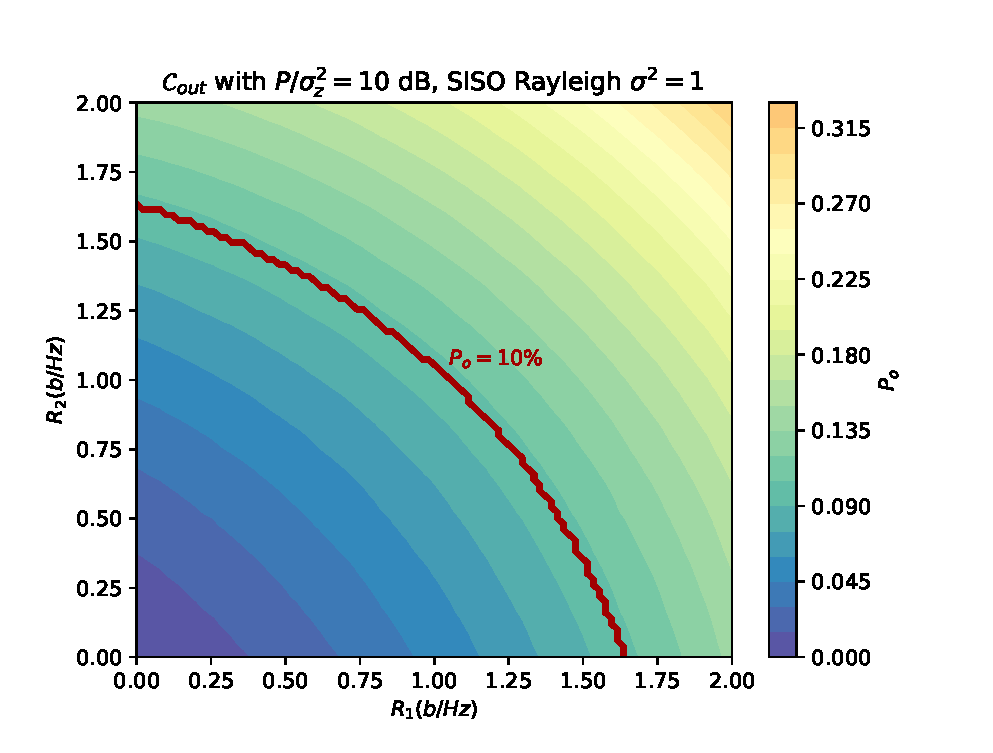
\includegraphics[width=\columnwidth]{paretoPo}   
    \end{figure}
 \end{column}
 
 \begin{column}{4cm}
    \begin{figure}
        \centering
        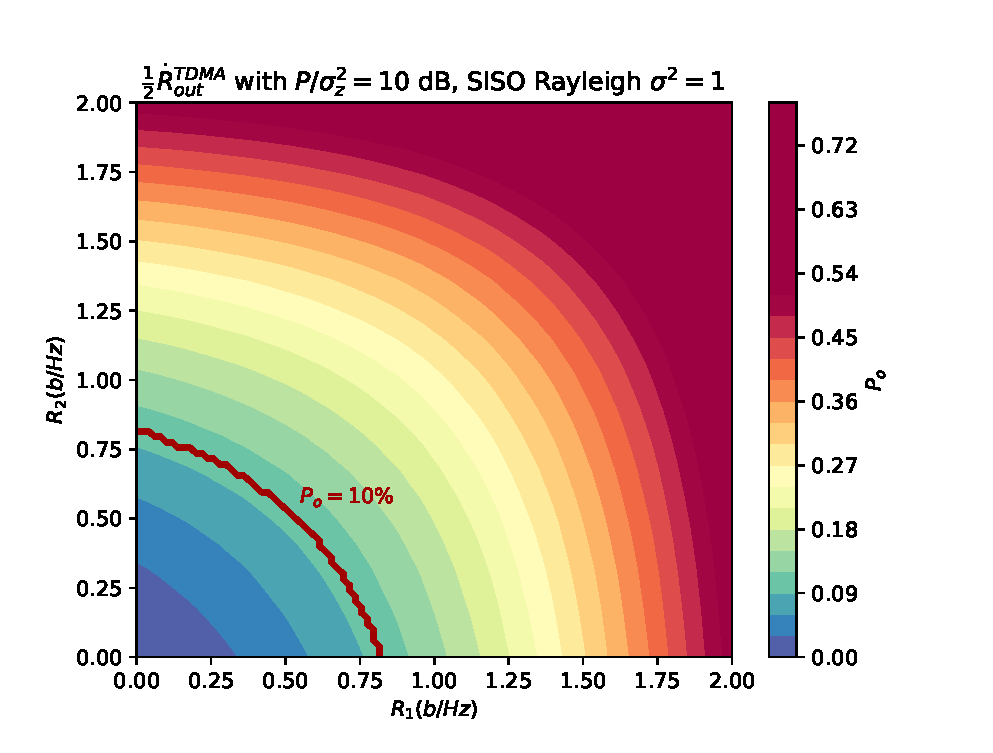
\includegraphics[width=\columnwidth]{paretoPoTDMA}   
    \end{figure}
 \end{column}
 
 \begin{column}{4cm}
    \begin{figure}
        \centering
        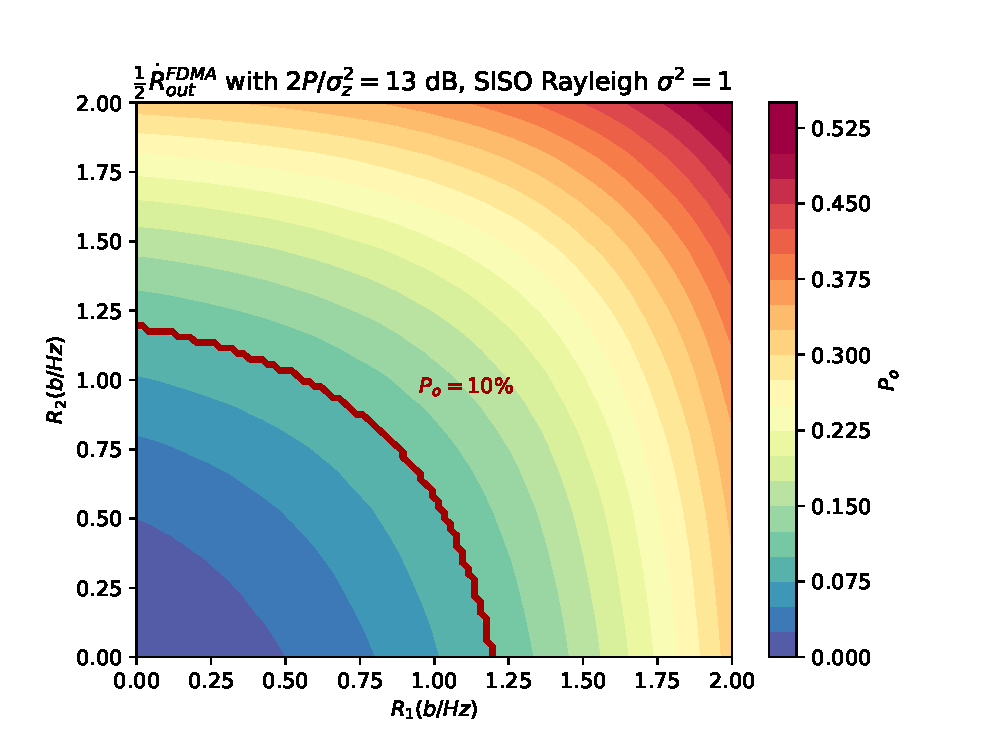
\includegraphics[width=\columnwidth]{paretoPoFDMA}   
    \end{figure}
 \end{column}
\end{columns}
\pagebreak

\begin{theorem}[Union Bound]
 In general $P_o\leq {\displaystyle\sum_{i\in\mathrm{system}}} P_o^{(i)}$. For very small $P_o^{(i)}$, $P_o\approx {\displaystyle\sum_{i\in\mathrm{system}}} P_o(i)$
\end{theorem}
\begin{itemize}
        \item Analysis of Orthogonal schemes\\ \ \\   
        
            \begin{itemize}
                \item Suppose all users have equal average SINR $\overline{\gamma}$\\ \ \\
                \item Given single-user Outage Capacity $C_{out}(\overline{\gamma},P_o)$\\ \ \\
                \item Defining system outage $\triangleq$ \textit{at least one} subchannel is in outage.\\ \ \\
                \item The $K$-user Orthogonal MAC Outage Capacity is
                $$\approx\frac{1}{K}C_o(\textcolor{FFucsia}{K}\overline{\gamma},\textcolor{ARust}{\frac{1}{K}}P_o)$$
        \end{itemize}
        
    \pagebreak
     \item Arbitrary schemes (capacity SIC and non-orthogonal achievable)\\ \ \\
     \begin{itemize}
     \begin{columns}
      \begin{column}{6cm}
       \item High SNR$\to$ Opportunistic Diversity    
            \begin{figure}
            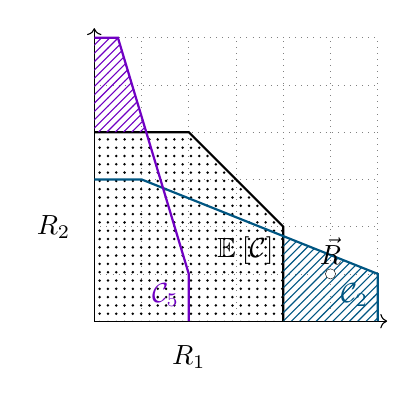
\begin{tikzpicture}[scale=.6]
                \draw[help lines,color=gray,dotted] (0,0) grid (6,6);
                \draw [->] (0,0) -- (0,6.2);
                \draw [->] (0,0) -- (6.2,0);
                \node [anchor=north] at (2,-0.3) {$R_1$}; 
                \node [anchor=east] at (-0.3,2) {$R_2$}; 
%                 \foreach \x in {0,1,...,4} { \node [anchor=north] at (\x,-0.3) {\tiny \x}; }
%                 \foreach \y in {0,1,...,4} { \node [anchor=east] at (-0.3,\y) {\tiny \y}; }        
         \draw[color=black,thick] (4,0) -- (4,2) -- (2,4) -- (0,4);       
         \fill[pattern=dots] (0,0) -- (4,0) -- (4,2) -- (2,4) -- (0,4);
         \node[anchor= north east,color=black] at (4,2) {$\Ex{}{\mathcal{C}}$};
         \draw[color=VCobalt,thick] (6,0) -- (6,1) -- (1,3) -- (0,3);
         \fill[pattern=north east lines,pattern color=VCobalt] (4,0) --  (6,0) -- (6,1) -- (4,1.8);
         \node[anchor= north east,color=VCobalt] at (6,1) {$\mathcal{C}_2$};
         \draw[color=FFucsia,thick] (2,0) -- (2,1) -- (.5,6) -- (0,6);      
         \fill[pattern=north east lines,pattern color=FFucsia] (0,4) -- (1.1,4) -- (.5,6) -- (0,6); 
         \node[anchor= north east,color=FFucsia] at (2,1) {$\mathcal{C}_5$};
         \draw[color=black,thin] (5,1) circle (.1);
         \fill[color=white,thin] (5,1) circle (.1);
         \node[anchor=south] at (5,1) {$\vec{R}$};
            \end{tikzpicture}
            \end{figure}
            $$\vec{R}\in\mathcal{C}_{out},\notin\Ex{}{\mathcal{C}}$$
      \end{column}
      \begin{column}{6cm}
        \item Low SNR$\simeq$ orthogonal
            \begin{figure}
                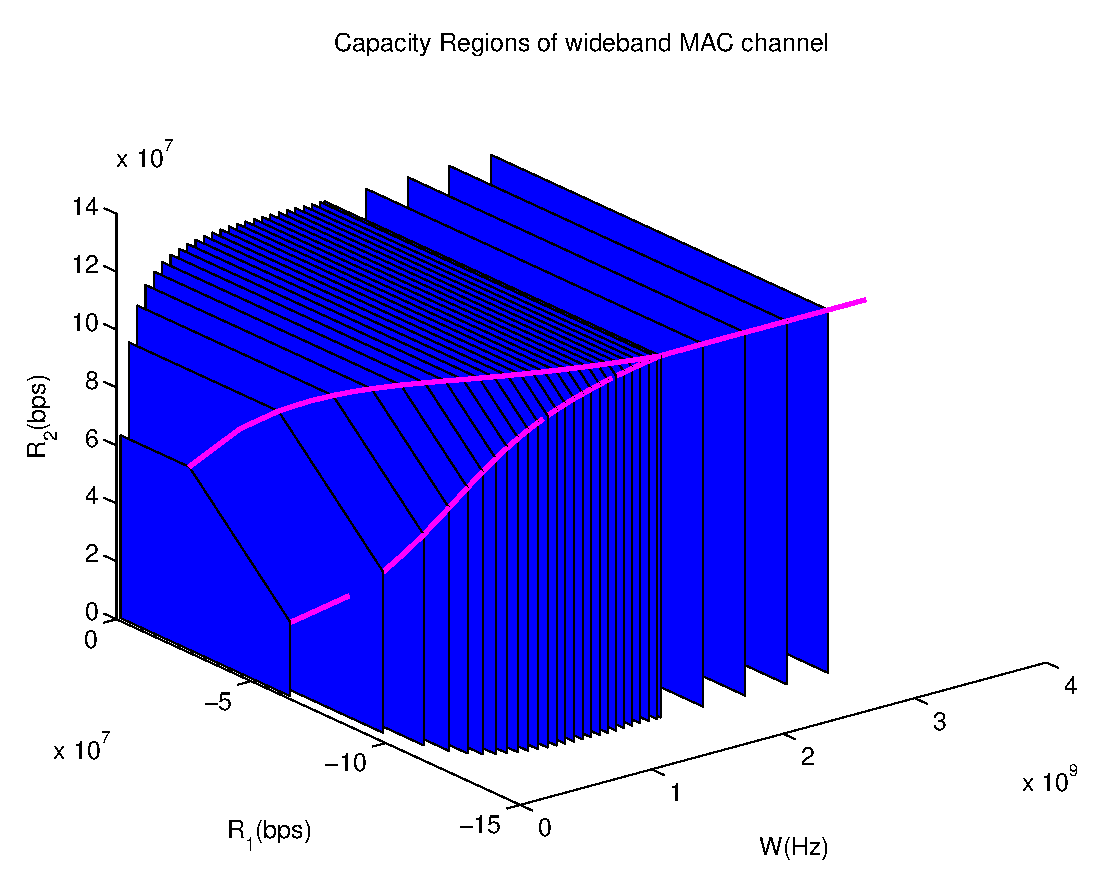
\includegraphics[width=.9\columnwidth]{capacityPanelsHybridCeiled}
%                         \caption{}
            \end{figure}
            $$ \lim_{\frac{P}{N_o}\to 0} \mathcal{C} = \textnormal{TDMA square}$$
      \end{column}
     \end{columns}
        \end{itemize}
    \end{itemize}
}

\frame[allowframebreaks]{\frametitle{\small Fast Fading MAC Channel Ergodic Rate Region}
     \begin{itemize}
        \item Each cut-set maximum sum rate is averaged \textit{separately}
            $$\sum_{k\in\mathcal{S}}R_k \leq \Ex{\Hb_{tot}}{\mathrm{CSB}_{AWGN}(\mathcal{S})}$$
        \item Orthogonal schemes cannot achieve maximum sum-rate
            $$\Ex{\Hb_{tot}}{\sum\frac{1}{K} B\log(1+\frac{P|h|^2}{\frac{B}{K}N_o})}=\Ex{\Hb_{tot}}{B\log(1+\frac{KP|h|^2}{BN_o})}$$
            $$<\Ex{\Hb_{tot}}{B\log(1+\frac{\sum_{k=1}^{K}P|h|^2}{BN_o})}$$
        \item SIC is optimal
     \end{itemize} 
     }

% \frame[allowframebreaks]{\frametitle{\small Homework: Wideband MAC Channels}
% \begin{homework}
%     Prove that FDMA achieves the optimal rate-region asymptotically in a \textit{wideband} MAC channel
%     $$\lim_{B\to\infty} \mathcal{R}_{FDMA} = \lim_{B\to\infty} \mathcal{C} $$
% \end{homework}
% }

\end{document}


